\documentclass[a4j,twoside,openright,11pt]{jarticle}
%
\usepackage{amsmath,amssymb}
\usepackage{bm}
\usepackage{graphicx}
\usepackage{ascmac}
\usepackage{listliketab}
\usepackage{url}
\usepackage{listings}

\setlength{\textwidth}{15.92cm}
\setlength{\oddsidemargin}{0mm}
\setlength{\evensidemargin}{0mm}
\setlength{\topmargin}{-1cm}
\setlength{\textheight}{23.5cm}
\setlength{\footskip}{18mm}

%
\pagestyle{plain}
\makeatletter
  \def\@maketitle{%
  \newpage\null
  \vskip 2em%
  \begin{center}%
  \let\footnote\thanks
    {\Large \@title \par}%
    \vskip 1.5em%
  \end{center}% 追加
  \begin{flushright}
        \@author
  \end{flushright}
  \begin{flushright}% 追加
    {\large \@date}%
  \end{flushright}%
  \par\vskip 1.5em}
\makeatother

\title{伝熱実験\\--熱電対を使った温度計測と熱伝導実験及び熱交換器実験--\\1.熱伝導実験}
\author{九州工業大学 機械知能工学科 機械コース\\3年 学籍番号:13104069 坂本 悠作}
\date{
実験日1:平成27年7月\,\,\,\,1日\\
提出日 :平成27年7月15日
}
\begin{document}
\maketitle
\newpage

\section{目的}
円柱内の1次元定常熱伝導実験からフーリエの法則について学ぶ
\section{フーリエの法則}
熱伝導は、温度分布の存在する物体、主として固体内において、温度差より熱エネルギーが高温側から低温側へ移動する現象である。物体内の単位面積を単位時間に通過する熱量$q[W/m^2]$(熱流速)は、一般に熱の流れる方向の温度勾配dT/dx[K/m]に比例する。この法則をフーリエの法則という。
\begin{eqnarray}
q = -\lambda \frac{dT}{dx}
\end{eqnarray}


\section{実験方法}
実験に試用するブロック(金属円柱:外形50[mm],高さ60[mm])は、銅、アルミニウム、黄銅の3種類である。ただし、どれがどの材料かは特定できないようにしている。実験では、任意の選択した1つの試験ブロックの下面を電気加熱した銅製ブロックに接触させて加熱し、上面を水道水によって冷却する。円柱側面は断熱材で断熱されているので、熱は下面から上面へ1方向(1次元的)に伝わる。軸方向に5箇所開けられた穴に挿入したT型熱電対で中心の温度分布を測定し記録する。

\section{実験手順}
\begin{enumerate}
\item 試験ブロックを加熱し、中心5点及び、冷却水の温度を測定する
\item 軸方向の温度分布をグラフに書き、ヒーター加熱量Qに対する勾配を最小二乗法によって求める
\item ヒーター加熱量から求まる熱流速(Q/A)と温度勾配との関係をグラフに表し、式1の関係について考察する
\item 上面の表面温度を外挿により求め、冷却水温度との差について比較する
\item 熱伝達について調べ、まとめる。
\end{enumerate}

\section{結果の整理}
\subsection{最小二乗法の計算}
最小二乗法は、誤差の自乗が最小になるように係数a,bを設定したものである。今回の実験では取得した値が5点であったので、5点の場合の計算方法を以下に示す。求めたい曲線をy=ax+bと仮定する今、データ点が$(x_1,y_1),(x_2,y_2),(x_3,y_3),(x_4,y_4),(x_5,y_5)$とすると、最小二乗法の考え方より、評価式Sが以下のようになる
\begin{eqnarray}
S &=& d_1^2 + d_2^2 + d_3^2 + d_4^2 + d_5^2 \nonumber\\
&=& (y_1-ax_1-b)^2 + (y_2-ax_2-b)^2 + (y_3-ax_3-b)^2 + (y_4-ax_4-b)^2 + (y_5-ax_5-b)^2\nonumber \\
&=&(y_1^2 + y_2^2 + y_3^2 + y_4^2 + y_5^2)\nonumber\\
&& +a^2(x_1^2 + x_2^2 + x_3^2 + x_4^2 + x_5^2)\nonumber\\
&& +5b^2\nonumber\\ 
&&- 2b(y_1 + y_2 + y_3 + y_4 + y_5)\nonumber\\
&& -2a(x_1y_1 + x_2y_2 + + x_3y_3 + + x_4y_4 + + x_5y_5) \nonumber\\
&&+ 2ab(x_1 + x_2 + x_3 + x_4 + x_5)
\end{eqnarray}

ここで、次の変数を宣言する
\begin{eqnarray}
A&=&(y_1^2 + y_2^2 + y_3^2 + y_4^2 + y_5^2)\nonumber\\
B&=&(x_1^2 + x_2^2 + x_3^2 + x_4^2 + x_5^2)\nonumber\\ 
C&=&(y_1 + y_2 + y_3 + y_4 + y_5)\nonumber\\
D&=&(x_1y_1 + x_2y_2 + + x_3y_3 + + x_4y_4 + + x_5y_5) \nonumber\\
E&=&(x_1 + x_2 + x_3 + x_4 + x_5)\nonumber\\
S&=&A+a^2B+5b^2-2bC-2aD+2abE
\end{eqnarray}
この評価式が最小となるように偏微分すると、
\begin{eqnarray}
\frac{\partial S}{\partial a} = 2aB-2D+2bE = 0\nonumber\\
\frac{\partial S}{\partial b} = 10b-2C+2aE  = 0\nonumber
\end{eqnarray}
これを解いて、
\begin{eqnarray}
a=\frac{5D-CE}{5B-E^2}\nonumber\\
b=\frac{BC-DE}{5B-E^2}
\end{eqnarray}

最小二乗法の計算によって、以下の式が求められた。
\begin{eqnarray}
y&=&-0.092x+302.45\\
y&=&-0.1315x+305.887\\
y&=&-0.202x+311.63\\
y&=&-0.253x+316.395
\end{eqnarray}

\begin{figure}[htbp]
\begin{center}
  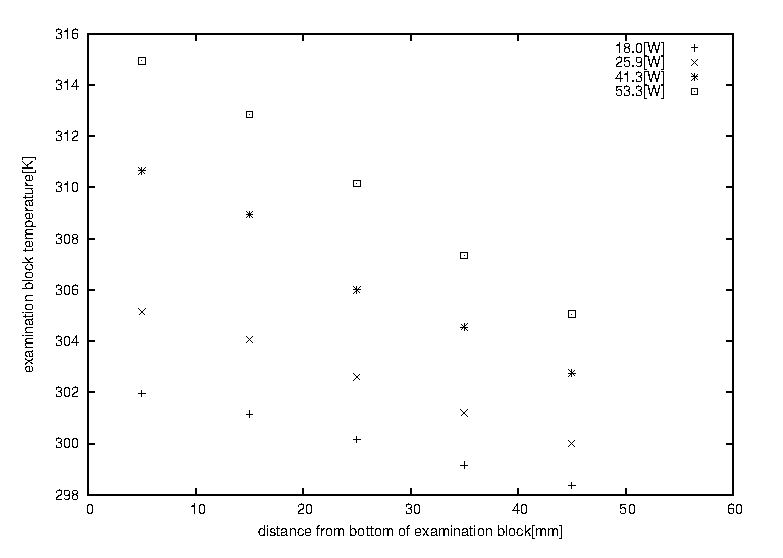
\includegraphics[width=12cm]{./fulie/data.eps}
\end{center}
\caption{軸方向温度分布}
\end{figure}

\begin{figure}[htbp]
\begin{center}
  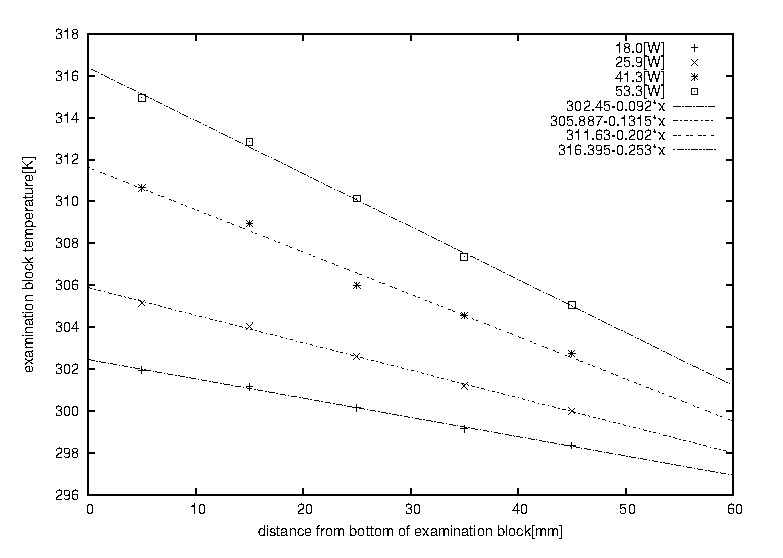
\includegraphics[width=12cm]{./fulie/data2.eps}
\end{center}
\caption{軸方向温度分布(最小二乗法)}
\end{figure}

\section{実験結果1−3のまとめ}
実験結果より得られたデータから、熱伝導率を導出する。前節の最小二乗法から、近似直線の傾きがわかるので、これを温度勾配[K/m]とした。
\begin{eqnarray}
熱流速[W/m^2] &=& ヒーター加熱量[W] / 断面積[m^2]\nonumber\\
              &=& 18.0/(0.025^2\pi)\nonumber\\
              &=& 9167.3[W/m^2]
\end{eqnarray}
熱伝導率は、次のように求めた。
\begin{eqnarray}
熱伝達率[W/(m\cdot K)] &=& 熱流速[W/m^2] / 温度勾配[K/m]\nonumber\\
                       &=& 9167.3/92\nonumber\\
                       &=& 99.64[W/(m\cdot K)]
\end{eqnarray}

この熱伝達率の平均を求めると、$102.84[W/(m\cdot K)]$を得た。よって、銅・アルミニウム・黄銅のいずれかだとすれば、この試験片は黄銅であることがわかる。

\begin{table}[htb]
\begin{center}
  \caption{熱伝達率の物質値概要}
  \begin{tabular}{lc}
    物質&熱伝達率$[W/(m\cdot K)]$\\
\hline
    銅&398\\
    アルミニウム&237\\
    黄銅&121\\
\hline
  \end{tabular}
\end{center}
\end{table}

\section{冷却水温との差}

試験ブロックの最上端の温度を求めるために、最小自乗法によって求めた式にx=60を代入する。
\begin{eqnarray}
y&=&-0.092x+302.45 = 296.93\\
y&=&-0.1315x+305.887 = 297.997\\
y&=&-0.202x+311.63 = 299.51\\
y&=&-0.253x+316.395 = 301.22
\end{eqnarray}
水温は294.65K(21.5℃)であるので、ブロック最上端の温度と水温に温度差が残っていることがわかる。

\section{参考文献}
\begin{enumerate}
\item \url{http://szksrv.isc.chubu.ac.jp/lms/lms1.html#section2}
\end{enumerate}
\section{参考資料}
今回の実験で最小二乗法を計算するために作成したプログラムを参考として添付します。
\small
\begin{verbatim}
/*-----------------------------------------------------
title:最小二乗法プログラム
author:yusaku sakamoto
last update:2015.07.10
mail:n104069y@mail.kyuteck.jp
how to use:
このプログラムは、第1列に横軸データ、2列目以降に縦軸データが入っているデータファイルを読み取ることを前提として作った最小二乗法の計算プログラムです。

コンパイルはg++を用いて行います。
$ make clean
$ make

で行って下さい。
実行方法は、行数×列数を引数として設定して下さい。
$ ./main 行数 列数 ファイル名
[例]
$ ./main 5 5 ../data.dat
------------------------------------------------------*/
#include <iostream>
#include <fstream>
#include <stdlib.h>
using namespace std;

#define BUF 20

int main(int argc,char *argv[])
{
  //引数の文字列を数字に変換
  //------------------------------------------------------
  const int row = atoi(argv[1]);
  const int column = atoi(argv[2]);
  const char *filename = argv[3];

  //ファイル読み取り用プログラム
  //------------------------------------------------------
  int i,j;
  double figure[row*column];
  fstream file;
  char character;
  char str[ row*column ][BUF];

  file.open(filename,ios::in);
  if( !file.is_open() ) perror("file open error");

  i=j=0;

  while(  file.read(&character, sizeof(character)) )
	{
	  if(character == '\t' || character == '\n'){
		figure[i] = atof(str[i]);
		i++;
		j=0;
	  }
	  else str[i][j++] = character;
	}
  file.close();

  //最小二乗法計算
  //------------------------------------------------------
  double x[row];
  double y[column-1][row];
  double A=0,B=0,C=0,D=0,E=0;
  double a[column-1];
  double b[column-1];
  int k;
  i=j=0;

  for(i=0;i<row;i++){
	x[i] = figure[j++];
	for(k=0;k<column-1;k++) y[k][i] = figure[j++];
  }

  for(j=0;j<column-1;j++){
	A=0;
	B=0;
	C=0;
	D=0;
	E=0;

	for(i=0;i<row;i++){
	  A += y[j][i]*y[j][i];
	  B += x[i]*x[i];
	  C += y[j][i];
	  D += x[i]*y[j][i];
	  E += x[i];
	}

	a[j] = (row*D-C*E)/(row*B-E*E);
	b[j] = (B*C-D*E)/(row*B-E*E);

	cout << "第" << j+2 << "列目の計算結果" << endl;
	cout << "\t---->>a:" << a[j] << endl;
	cout << "\t---->>b:" << b[j] << endl;
  }

  return 0;
}
\end{verbatim}
\normalsize
\end{document}
